\phantomsection

\chapter{Exploitation}
\markboth{Exploitation}{}
La fase di acquisizione della macchina target è stata svolta a partire dalle informazioni ricavate nell'ambito del \emph{Vulnerability Mapping}. Dal momento che un'exploitation esaustiva fa sia uso di tool automatizzati che di tecniche manuali volte allo sfruttamento delle vulnerabilità presenti sull'asset, il presente capitolo è stato suddiviso in due parti, ciascuna dedicata alla trattazione di una specifica strategia.
\section{Tecniche automatiche di exploitation}
Il processo di exploitation può essere automatizzato mediante appositi tool che mettono a disposizione \emph{exploit} e \emph{payload} pronti all'uso. Nei seguenti paragrafi verrà trattato l'utilizzo di \emph{Metasploit (v. 6.3.16-dev)}, uno degli strumenti più popolari, e del relativo \emph{front-end} \emph{Armitage (v. 20220123)}. 
\subsection{Metasploit}
Effettuare la fase di \emph{exploitation} mediante la console di \emph{Metasploit} risulta essere un'operazione piuttosto onerosa se non si conosce l'exploit da utilizzare. Il tool mette a disposizione una funzionalità di ricerca che consente di individuare l'exploit da utilizzare mediante delle parole chiave. Nell'ambito del processo effettuato sono state eseguite diverse ricerche relative alle vulnerabilità individuate che, avendo una severity bassa ed essendo principalmente basate sul trapelamento di informazioni sulla versione del \emph{Web Server}, non hanno portato a particolari riscontri. Nelle successive sezioni sono riportati dei resoconti sulle ricerche effettuate in merito alle vulnerabilità riportate dai diversi tool.
\subsubsection{OpenVAS}
Le vulnerabilità rilevate da \emph{OpenVAS} sono:
\begin{itemize}
    \item \textbf{ICMP Timestamp Reply Information Disclosure}: per questa vulnerabilità \emph{OpenVAS} ha riportato la \emph{CVE-1999-0524}. Una ricerca in merito su \emph{Metasploit} non ha prodotto alcun risultato (figura \ref{fig:metasploit_trid});
    \begin{figure}[h]
        \centering
        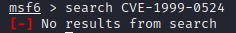
\includegraphics[scale=1]{capitoli/images/metasploit_trid.png}
        \caption{Risultati della ricerca di un exploit per \emph{CVE-1999-0524}}
        \label{fig:metasploit_trid}
    \end{figure}
    \item \textbf{TCP Timestamps Information Disclosure}: per questa vulnerabilità \emph{OpenVAS} non ha riportato alcuna \emph{CVE}. 
\end{itemize}

\subsubsection{Nessus}
Escludendo i falsi positivi, le vulnerabilità riportate da \emph{Nessus} sono:
\begin{itemize}
    \item \textbf{Browsable Web Directories}: per questa vulnerabilità \emph{Nessus} non ha riportato alcuna \emph{CVE}. In generale, tale tipo di vulnerabilità rappresenta un punto di partenza per un'esplorazione manuale delle directory del Server;
    \item \textbf{Web Application Potentially Vulnerable to Clickjacking}: per questa vulnerabilità \emph{Nessus} non ha riportato alcuna \emph{CVE}. È stata, in ogni caso, svolta una ricerca volta all'identificazione di un exploit da utilizzare, tuttavia l'unico risultato ottenuto non risulta essere pertinente al contesto esaminato, in quanto fa riferimento ad una distribuzione di \emph{firewall} e \emph{router} (figura \ref{fig:metasploit_clickjacking}) 
    \begin{figure}[h]
        \centering
        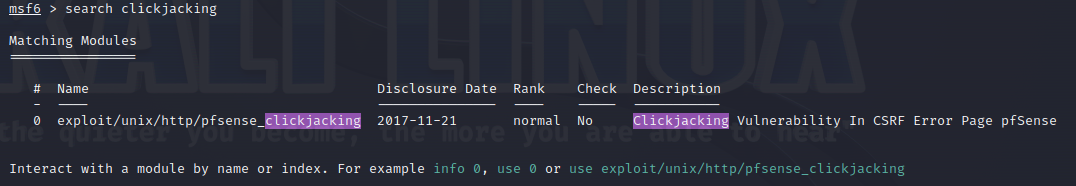
\includegraphics[scale=0.4]{capitoli/images/metasploit_clickjacking.png}
        \caption{Risultati della ricerca di un exploit per il \emph{clickjacking}}
        \label{fig:metasploit_clickjacking}
    \end{figure}
\end{itemize}
\subsubsection{Nikto2}
Le vulnerabilità rilevate da \emph{Nikto2} sono le seguenti:
\begin{itemize}
    \item \textbf{Assenza dell'opzione X-Frame-Options nel'header come protezione dal clickjacking}: tale vulnerabilità risulta essere analoga a quella trattata in precedenza;
    \item \textbf{Gli ETag della risposta espongono informazioni relative al numero dell'inode}: per questa vulnerabilità \emph{OpenVAS} ha riportato la \emph{CVE-2003-1418}. Una ricerca in merito su \emph{Metasploit} non ha prodotto alcun risultato (figura \ref{fig:metasploit_trid});
    \begin{figure}[h]
        \centering
        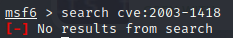
\includegraphics[scale=1]{capitoli/images/metasploit_etag.png}
        \caption{Risultati della ricerca di un exploit per \emph{CVE-2003-1418}}
        \label{fig:metasploit_etag}
    \end{figure}
    \item \textbf{La versione di Apache (2.4.38) risulta essere obsoleta}: per questa vulnerabilità \emph{OpenVAS} non ha riportato una \emph{CVE} di riferimento. È stata, in ogni caso, svolta una ricerca volta all'identificazione di un exploit da utilizzare, tuttavia non è stato ottenuto alcun risultato (figura \ref{fig:metasploit_apache})
    \begin{figure}[h]
        \centering
        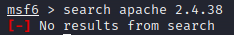
\includegraphics[scale=1]{capitoli/images/metasploit_apache.png}
        \caption{Risultati della ricerca di un exploit per \emph{Apache 2.4.38}}
        \label{fig:metasploit_apache}
    \end{figure}
\end{itemize}
Tutte le altre vulnerabilità non hanno una \emph{CVE} di riferimento e la maggior parte di queste non si prestano ad attacchi automatizzati in quanto fungono da punto di partenza per l'esplorazione del \emph{Web Server}. 

\subsubsection{OWASP ZAP}
L'unica vulnerabilità rilevata da \emph{OWASP ZAP} a non essere stata già rilevata è quella relativa all'assenza di un \emph{Content Security Policy} nell'header della risposta. Dal momento che l'assenza di tale header rende il \emph{Web Server} vulnerabile ad attacchi di tipo \emph{XSS}, è stata svolta una ricerca in merito a tale tipo di attacco. Nonostante i numerosi risultati (figura \ref{fig:metasploit_xss}), nessuno di questi risulta essere utilizzabile nel contesto in esame.
\begin{figure}[h]
    \centering
    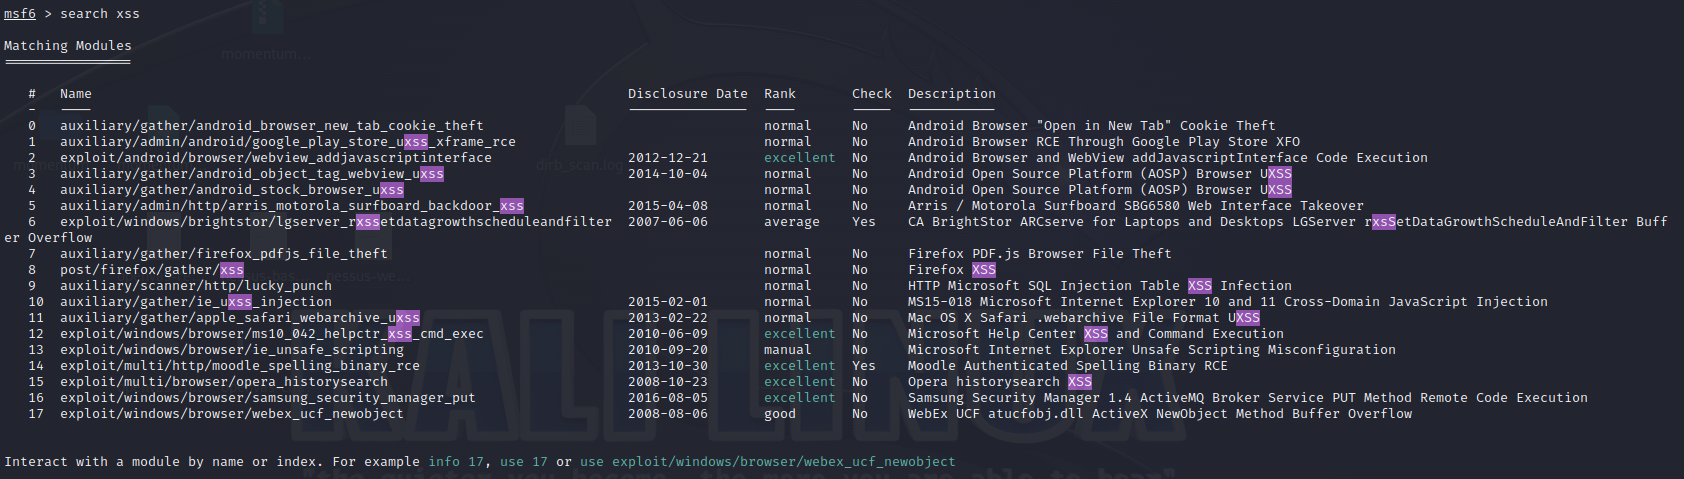
\includegraphics[scale=0.3]{capitoli/images/metasploit_xss.png}
    \caption{Risultati della ricerca di un exploit per \emph{XSS}}
    \label{fig:metasploit_xss}
\end{figure}

\subsubsection{Paros Proxy}
\emph{Paros Proxy} non ha rilevato ulteriori vulnerabilità rispetto a quelle trattate in precedenza. 
\subsection{Armitage}
Dal momento che la ricerca effettuata mediante la console di \emph{Metasploit} non ha portato alcun risultato, è stato utilizzato il tool \emph{Armitage} che funge da \emph{front-end} per \emph{Metasploit} e mette a disposizione un'utile funzionalità che consente di rilevare gli attacchi disponibili per un determinato asset e provare in \emph{flood} tutti i possibili \emph{exploit} e \emph{payload} al fine di tentare di stabilire una sessione verso l'asset stesso. Come si può dedurre dai report (reperibili all'interno della cartella \emph{`tools\_output/armitage-report'}) ed in particolare dal report \emph{`hailmary.log'}, neanche questa strategia ha portato all'individuazione di un \emph{exploit} in grado di sfruttare una vulnerabilità della macchina target. Al termine del processo, infatti, \emph{Armitage} notifica l'assenza di sessioni con la macchina target (figura \ref{fig:armitage}).
\begin{figure}[h]
    \centering
    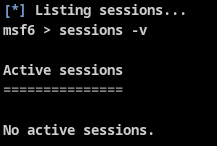
\includegraphics[scale=1]{capitoli/images/armitage.png}
    \caption{Risultato dell'esecuzione di \emph{Armitage}}
    \label{fig:armitage}
\end{figure}
\section{Tecniche manuali di exploitation}
Il fallimento delle tecniche automatiche di \emph{exploitation} ha reso necessario l'utilizzo di tecniche manuali volte all'individuazione di vulnerabilità da sfruttare. Tale fase è stata svolta tenendo in considerazione le informazioni apprese nell'ambito delle precedenti fasi; in particolare è stato fondamentale focalizzare l'attenzione sui servizi attivi della macchina e sulla vulnerabilità relativa al \emph{browsing} delle directory del \emph{Web Server}. 

\subsection{Browsing delle directory del \emph{Web Server}}
In fase di \emph{Vulnerability Mapping}, diversi tool hanno segnalato la possibilità di navigare le directory del \emph{Web Server}, riportandone alcune ritenute rilevanti; in particolare:
\begin{itemize}
    \item La directory \emph{10.0.2.4/css} contiene il file \emph{CSS} relativo alle pagine del sito;
    \item La directory \emph{10.0.2.4/img} contiene le quattro immagini mostrate nella \emph{Home Page} del sito;
    \item La directory \emph{10.0.2.4/js} contiene il file \emph{JavaScript `main.js'} all'interno del quale è definita la funzione che, al click dell'utente su un'immagine, effettua il \emph{redirect} alla pagina contenente i dettagli relativi all'opera d'arte visualizzata. 
    \end{itemize}
\begin{figure}[h]
    \centering
    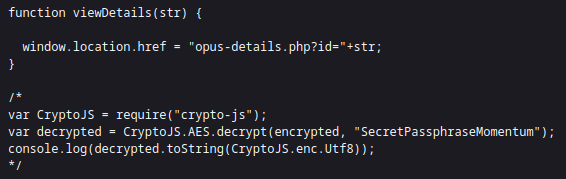
\includegraphics[scale=1]{capitoli/images/js.png}
    \caption{Contenuto dello script \emph{`main.js'}}
    \label{fig:js}
\end{figure}
L'aspetto più interessante di tale script (figura \ref{fig:js}) non risulta, tuttavia, essere la funzione \emph{`viewDetails'}, bensì la presenza di un commento che rappresenta probabilmente la prima informazione utile rilevata in fase di \emph{exploitation}. Tale commento, infatti, contiene la chiamata ad una funzione di decifratura (che fa uso dell'algoritmo \emph{AES}) alla quale viene passata in input, come secondo parametro, una password in chiaro: \emph{`SecretPassphraseMomentum'}.
\subsection{Utilizzo della password individuata}
Dopo aver individuato la password in chiaro all'interno del codice, è stato necessario comprendere se ed in che contesto fosse possibile utilizzarla. Non avendo rilevato, nell'ambito delle precedenti fasi, una schermata di \emph{Log In} sul \emph{Web Server}, è stata considerata l'idea che tale password potesse essere sfruttata per accedere al servizio \emph{SSH}. Non essendo a conoscenza degli \emph{username} degli utenti della macchina target, è stato tentato un accesso all'account di \emph{root}, senza, tuttavia, successo (figura \ref{fig:ssh_fail}). 
\begin{figure}[h]
    \centering
    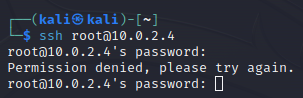
\includegraphics[scale=1]{capitoli/images/ssh_fail.png}
    \caption{Fallimento del \emph{log in SSH}}
    \label{fig:ssh_fail}
\end{figure}
Abbandonata l'idea di utilizzare tale password per accedere ad un servizio della macchina target, è stata considerata la possibilità di utilizzarla per decifrare eventuali dati cifrati. Le fasi finora considerate, non hanno rilevato la presenza di dati da decifrare, tuttavia nell'ambito di un \emph{Web Server} risulta lecito ipotizzare la presenza di \emph{cookie} eventualmente cifrati. Tramite \emph{Firefox} è possibile rilevare la presenza di un cookie cifrato nel momento in cui si visita la pagina \emph{`10.0.2.4/opus-details.php?id=demon'} (figura \ref{fig:cookie}).
\begin{figure}[h]
    \centering
    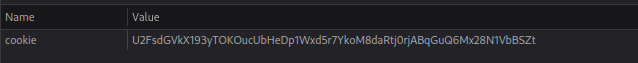
\includegraphics[scale=1]{capitoli/images/cookie.png}
    \caption{Cookie cifrato}
    \label{fig:cookie}
\end{figure}

Per decifrare il cookie individuato, usando la password \emph{`SecretPassphraseMomentum'}, è stato configurato un ambiente \emph{Node.js} in \emph{Kali} al fine di eseguire uno script (illustrato nella figura \ref{fig:decrypt} e reperibile nella cartella \emph{script}) analogo a quello individuato nei comenti di \emph{`main.js`}. L'output della sua esecuzione (riportato nella figura \ref{fig:decrypted}) comporta la stampa a schermo della stringa \emph{`auxerre-alienum\#\#'}.  
\begin{figure}[h]
    \centering
    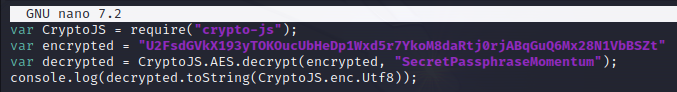
\includegraphics[scale=0.6]{capitoli/images/decrypt.png}
    \caption{Script per la decifratura del cookie}
    \label{fig:decrypt}
\end{figure}
\begin{figure}[h]
    \centering
    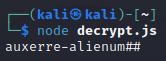
\includegraphics[scale=1]{capitoli/images/decrypted.png}
    \caption{Output della decifratura del cookie}
    \label{fig:decrypted}
\end{figure}
\subsection{Accesso al servizio \emph{SSH}}
La decifratura del \emph{cookie} individuato ha portato all'individuazione di una nuova stringa (\emph{`auxerre-alienum\#\#'}) avente le sembianze di una password. L'unico servizio individuato su cui risulta possibile utilizzare una password è \emph{SSH}, tuttavia manca il riferimento ad uno \emph{username} corrispondente. In assenza di ulteriori indizi, sono stati effettuati diversi tentativi di accesso, cercando di intuire lo \emph{username} dalla stringa. Osservandone la struttura, infatti, è possibile notare che essa sembri divisa in due parti dal carattere \emph{`-'}; risulta, dunque, lecito intuire che la prima parte rappresenti lo username, mentre la seconda parte la password (tale intuizione è avvalorata dalla presenza di due caratteri speciali). Il tentativo di accesso al servizio \emph{SSH} utilizzando \emph{`auxerre'} come username e \emph{`alienum\#\#'} come password non è, tuttavia, andato a buon fine. Le osservazioni evidenziate fino a questo momento non risultano, tuttavia, del tutto errate. In seguito a diversi tentativi, infatti, è stato confermato che la prima parte della stringa rappresenti lo \emph{username}, mentre la password è la stringa per intero. Come riportato nella figura \ref{fig:ssh_success}, utilizzando lo username \emph{`auxerre'} e la password \emph{`auxerre-alienum\#\#'}, si ottiene l'accesso alla macchina target, completando con successo la fase di \emph{exploitation}. 
\begin{figure}[h]
    \centering
    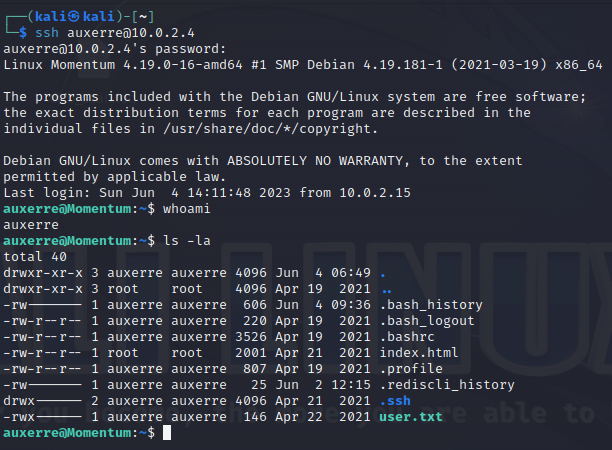
\includegraphics[scale=0.7]{capitoli/images/ssh_success.png}
    \caption{Accesso alla macchina target tramite il servizio \emph{SSH}}
    \label{fig:ssh_success}
\end{figure}
\subsection{Cross Site Scripting}
In fase di \emph{Vulnerability Mapping} il tool \emph{Paros Proxy} ha segnalato la possibilità di effettuare \emph{Cross Site Scripting} sulla pagina \emph{`http://10.0.2.4/opus-details.php'}.  
Sebbene l'accesso alla macchina target sia stato possibile grazie alla presenza di una password all'interno di uno script, al fine di svolgere una fase di \emph{exploitation} esaustiva, risulta utile tentare di sfruttare tale vulnerabilità. A tale scopo, è necessario preparare un \emph{URL} contenente uno script da iniettare nella pagina; il tool \emph{Paros Proxy}, nel report generato, fornisce un \emph{URL} di questo tipo: \emph{`http://10.0.2.4/opus-details.php?id=\%3CSCRIPT\%3Ealert\(\%22Paros\%22\);\%3C/SCRIPT\%3E'}. La figura \ref{fig:xss} mostra il risultato dell'iniezione dello script, che consiste in un semplice alert. Tale vulnerabilità risulta, dunque, sfruttabile e può portare al furto dei dati di sessione degli utenti del sito mediante, ad esempio, l'iniezione di script che prelevano i cookie e li inviano ad un server controllato da un attaccante.
\begin{figure}[h]
    \centering
    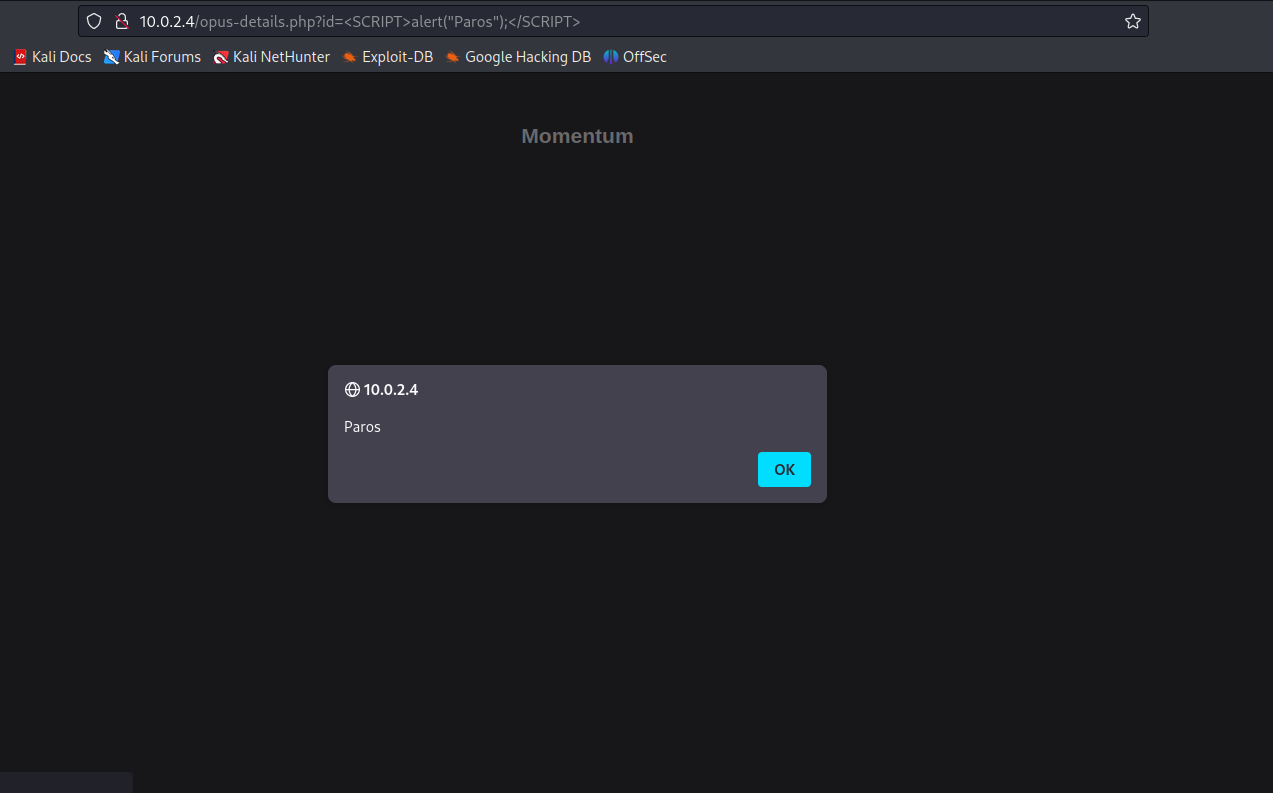
\includegraphics[scale=0.4]{capitoli/images/xss.png}
    \caption{Risultato dell'esecuzione del \emph{Cross Site Scripting}}
    \label{fig:xss}
\end{figure}
